ROS (Robotic Operating System) is an open source framework made toward robotic application.
The goal of ROS is to propose means to facilitate communication between processes,managing possibilities and make available working algorithms for everyone~\cite{quigley2009ros}.

This framework will be use in this project for communication and visualisation.

\subsection{How it works}

ROS is functioning with nodes, a master and slaves,the master is a ROS process and nodes can be programmed by anyone:

\begin{itemize}[label=$-$,itemsep=0cm,topsep=0cm]
\item The framework is available on many OS (operating system)such as Linux (CPU architecture: ARM x86 x64), Android , Windows, OSX;
\item The programming of the nodes can be done in multiple language : C++, Python, Java, Lua, Lisp, C\#, Go, R, Ruby (from the most supported to the least)
\item Nodes written in different languages can function together.
\end{itemize}

The communication with ROS works with topics,subscriber, and publisher, a publishing node will announce to the master that it is publishing over a topic and the subscribing node will say to the master that it want to listen to a topic. Then if the publisher and the subscriber are on the same topic, the master will transfer data in order for the two other node to communicate directly via TCP/IP or UDP (see figure~\ref{fig:rosTopic}).

\begin{figure}[H]
\centering
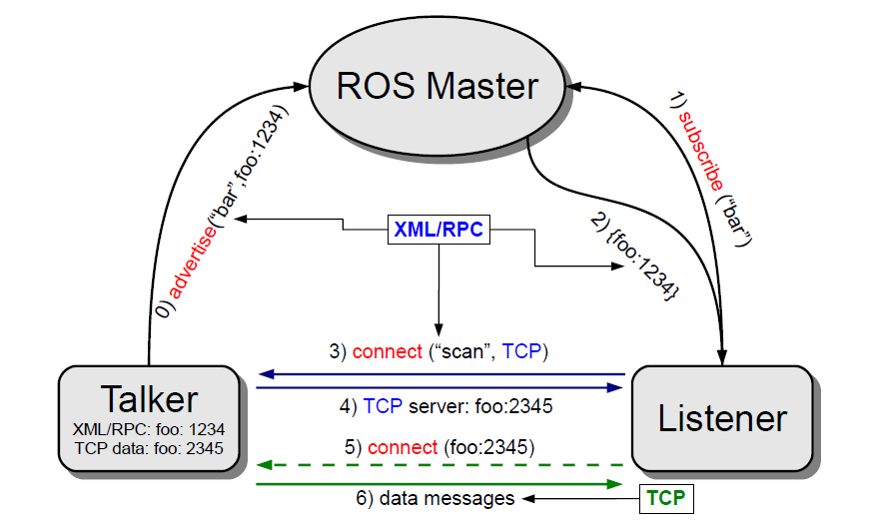
\includegraphics[scale=0.75]{ros_func.png}
\caption{Connection of nodes and topics \cite{rusu13ros}.}
\label{fig:rosTopic}
\end{figure}

ROS also facilitate the serialization of messages (conversion of the message into bytes):\\

\begin{minipage}[b]{0.8\textwidth}
\begin{itemize}[label={},itemsep=0cm,topsep=0cm]
\item std\_msgs/Header header
  \begin{itemize}[label={},itemsep=0cm,topsep=0cm]
  \item uint32 seq
  \item time stamp
  \item string frame\_id
   \end{itemize}
\item geometry\_msgs/Quaternion orientation
  \begin{itemize}[label={},itemsep=0cm,topsep=0cm]
  \item float64 x
  \item float64 y
  \item float64 z
  \item float64 w
  \end{itemize}
\end{itemize}
\end{minipage}


As it can be seen in the message example, a message can reference another message, in order to create message capable of transmitting complex data (an image with all its meta data).
This functionality of ROS permits a big modularity for the programmer, an easy passage from simulation to real via only changing topic names.

\subsection{ROS in the project}

For the simulation of the swarm slam project multiple nodes have been 
created in order to represent accurate communication and sensing.

\subparagraph*{IA\_MSGS}

ia\_msgs is an utility package to regroup created message in order to help to the communication of interval vector (in 2 and 3 dimension):\\

\begin{itemize}[label={},itemsep=0cm,topsep=0cm]
\item std\_msgs/Header header
  \begin{itemize}[label={},itemsep=0cm,topsep=0cm]
  \item uint32 seq
  \item time stamp
  \item string frame\_id
  \end{itemize}
\item ia\_msgs/IdInterval[] data
  \begin{itemize}[label={},itemsep=0cm,topsep=0cm]
  \item uint8 id
  \item ia\_msgs/Interv[] data
    \begin{itemize}[label={},itemsep=0cm,topsep=0cm]
    \item geometry\_msgs/Point position
      \begin{itemize}[label={},itemsep=0cm,topsep=0cm]
      \item float64 x
      \item float64 y
      \item float64 z
      \end{itemize}
    \item float64 width
    \item float64 height
    \end{itemize}
  \end{itemize}
\end{itemize}
\subparagraph*{RVIZ\_IA\_PLUGIN}
\subparagraph*{IA\_SLAM}
\subparagraph*{ROBOT\_SIMU}
\subparagraph*{BEACON\_SIMU}
\subparagraph*{TALK\_SIMU}
\subparagraph*{IA\_CONTROLLER}


